%%
%% This is file `sample-sigconf.tex',
%% generated with the docstrip utility.
%%
%% The original source files were:
%%
%% samples.dtx  (with options: `all,proceedings,bibtex,sigconf')
%% 
%% IMPORTANT NOTICE:
%% 
%% For the copyright see the source file.
%% 
%% Any modified versions of this file must be renamed
%% with new filenames distinct from sample-sigconf.tex.
%% 
%% For distribution of the original source see the terms
%% for copying and modification in the file samples.dtx.
%% 
%% This generated file may be distributed as long as the
%% original source files, as listed above, are part of the
%% same distribution. (The sources need not necessarily be
%% in the same archive or directory.)
%%
%%
%% Commands for TeXCount
%TC:macro \cite [option:text,text]
%TC:macro \citep [option:text,text]
%TC:macro \citet [option:text,text]
%TC:envir table 0 1
%TC:envir table* 0 1
%TC:envir tabular [ignore] word
%TC:envir displaymath 0 word
%TC:envir math 0 word
%TC:envir comment 0 0
%%
%% The first command in your LaTeX source must be the \documentclass
%% command.
%%
%% For submission and review of your manuscript please change the
%% command to \documentclass[manuscript, screen, review]{acmart}.
%%
%% When submitting camera ready or to TAPS, please change the command
%% to \documentclass[sigconf]{acmart} or whichever template is required
%% for your publication.
%%
%%
\documentclass[sigconf]{acmart}
%%
%% \BibTeX command to typeset BibTeX logo in the docs
\AtBeginDocument{%
  \providecommand\BibTeX{{%
    Bib\TeX}}}

%% Rights management information.  This information is sent to you
%% when you complete the rights form.  These commands have SAMPLE
%% values in them; it is your responsibility as an author to replace
%% the commands and values with those provided to you when you
%% complete the rights form.
\setcopyright{acmlicensed}
\copyrightyear{2025}
\acmYear{2025}
%\acmDOI{XXXXXXX.XXXXXXX}
%% These commands are for a PROCEEDINGS abstract or paper.
\acmConference[EnergySP '25]{ACM SIGEnergy Workshop on Cybersecurity and Privacy of Energy Systems}{June 17, 2025}{Rotterdam, NL}
%%
%%  Uncomment \acmBooktitle if the title of the proceedings is different
%%  from ``Proceedings of ...''!
%%
%%\acmBooktitle{Woodstock '18: ACM Symposium on Neural Gaze Detection,
%%  June 03--05, 2018, Woodstock, NY}
\acmISBN{978-1-4503-XXXX-X/2018/06}


%%
%% Submission ID.
%% Use this when submitting an article to a sponsored event. You'll
%% receive a unique submission ID from the organizers
%% of the event, and this ID should be used as the parameter to this command.
%%\acmSubmissionID{123-A56-BU3}

%%
%% For managing citations, it is recommended to use bibliography
%% files in BibTeX format.
%%
%% You can then either use BibTeX with the ACM-Reference-Format style,
%% or BibLaTeX with the acmnumeric or acmauthoryear sytles, that include
%% support for advanced citation of software artefact from the
%% biblatex-software package, also separately available on CTAN.
%%
%% Look at the sample-*-biblatex.tex files for templates showcasing
%% the biblatex styles.
%%

%%
%% The majority of ACM publications use numbered citations and
%% references.  The command \citestyle{authoryear} switches to the
%% "author year" style.
%%
%% If you are preparing content for an event
%% sponsored by ACM SIGGRAPH, you must use the "author year" style of
%% citations and references.
%% Uncommenting
%% the next command will enable that style.
%%\citestyle{acmauthoryear}

\usepackage{listings}
\lstset{
basicstyle=\small\ttfamily,
columns=flexible,
breaklines=true
}


%%
%% end of the preamble, start of the body of the document source.
\begin{document}

%%
%% The "title" command has an optional parameter,
%% allowing the author to define a "short title" to be used in page headers.
\title{Charging Communication Sniffing and Man-in-the-Middle Attacks}

%%
%% The "author" command and its associated commands are used to define
%% the authors and their affiliations.
%% Of note is the shared affiliation of the first two authors, and the
%% "authornote" and "authornotemark" commands
%% used to denote shared contribution to the research.
\author{Lukas Eder}
\authornote{Both authors contributed equally to this research.}
\email{lukas.eder@carissma.eu}
\author{Jakob Löw}
\authornotemark[1]
\email{jakob.loew@thi.de}
\orcid{0009-0006-7088-8684}
\affiliation{%
  \institution{Technische Hochschule Ingolstadt}
  \city{Ingolstadt}
  %\state{Bavaria}
  \country{Germany}
}

\author{Hans-Joachim Hof}
\affiliation{%
  \institution{Technische Hochschule Ingolstadt}
  \city{Ingolstadt}
  \country{Germany}}
\email{hof@thi.de}
\orcid{0000-0002-6930-9271}

%%
%% By default, the full list of authors will be used in the page
%% headers. Often, this list is too long, and will overlap
%% other information printed in the page headers. This command allows
%% the author to define a more concise list
%% of authors' names for this purpose.
\renewcommand{\shortauthors}{Eder and Loew et al.}

%%
%% The abstract is a short summary of the work to be presented in the
%% article.
\begin{abstract}
In recent years an increasing amount of electric vehicle fast charging stations have been built to meet the growing demand from rising electric vehicle numbers.
The standard for fast charging communication in europe is ISO\,15118.
In theory the standard includes security controls for authentication and transport encryption.
In reality difficulties with implementing those security controls as well as insecure design within the standard lead to multiple possible attack vectors compromising the confidentiality and authenticity of charging communication sessions.
The goal of this research is to present different approaches towards performing sniffing and man-in-the-middle attacks against charging communication.
We also provide a novel approach, which does not rely on race conditions and thus is more reliable than previous approaches.
\end{abstract}

%%
%% The code below is generated by the tool at http://dl.acm.org/ccs.cfm.
%% Please copy and paste the code instead of the example below.
%%
\begin{CCSXML}
<ccs2012>
   <concept>
       <concept_id>10002978.10003001.10003003</concept_id>
       <concept_desc>Security and privacy~Embedded systems security</concept_desc>
       <concept_significance>500</concept_significance>
       </concept>
   <concept>
       <concept_id>10002978.10003014.10003015</concept_id>
       <concept_desc>Security and privacy~Security protocols</concept_desc>
       <concept_significance>300</concept_significance>
       </concept>
   <concept>
       <concept_id>10010583.10010662.10010663.10010664</concept_id>
       <concept_desc>Hardware~Batteries</concept_desc>
       <concept_significance>300</concept_significance>
       </concept>
 </ccs2012>
\end{CCSXML}

\ccsdesc[500]{Security and privacy~Embedded systems security}
\ccsdesc[300]{Security and privacy~Security protocols}
\ccsdesc[300]{Hardware~Batteries}

%%
%% Keywords. The author(s) should pick words that accurately describe
%% the work being presented. Separate the keywords with commas.
\keywords{Security, Charging, ISO\,15118, Electric Vehicles, CCS, Fast Charging, Rapid Charging, Powerline}
%% A "teaser" image appears between the author and affiliation
%% information and the body of the document, and typically spans the
%% page.
\iffalse
\begin{teaserfigure}
  \includegraphics[width=\textwidth]{sampleteaser}
  \caption{Seattle Mariners at Spring Training, 2010.}
  \Description{Enjoying the baseball game from the third-base
  seats. Ichiro Suzuki preparing to bat.}
  \label{fig:teaser}
\end{teaserfigure}
\fi

\received{01 April 2025}
%\received[revised]{12 March 2009}
%\received[accepted]{5 June 2009}

%%
%% This command processes the author and affiliation and title
%% information and builds the first part of the formatted document.
\maketitle

\section{Introduction}
With the increasing spread of electric mobility, the IT security of the charging process is becoming increasingly important. Standards such as ISO\,15118 define secure communication protocols between an electric vehicle (EV) and an electric vehicle supply equipment (EVSE), but manufacturer specific implementations often remain undocumented. This makes it difficult to analyze potential vulnerabilities and security risks, especially for proprietary protocols that are used outside of standardized solutions.

In order to identify and reduce potential security risks in charging communication, it is necessary to extract communication data directly from real charging processes. This requires sniffing the communication between the EV and the EVSE. However, existing man-in-the-middle devices are often expensive and thus difficult to access. Other solutions, which are shown later in this paper, are not reliable or difficult to use. Therefore, the aim of this paper is to show a cost-efficient, accessible, and reliable solution for sniffing the charging communication. This allows both proprietary protocols to be analyzed and standard implementations to be verified.

In the scope of this paper, different sniffing approaches are explained and a method for sniffing the communication between EV and EVSE with minimal hardware and configuration effort is further investigated and implemented. The developed solution is reliable and suitable for use in laboratory environments as well as in real-world scenarios. It provides a basis for further security analysis in the field of electric mobility.

\section{Charging Communication Technology}
This chapter focuses on some aspects of EV charging communication that form the basis of this paper. First, the physical conditions, in particular the Combined Charging System (CCS) and Powerline Communication (PLC), are analyzed. This is followed by an examination of the communication process, looking at low-level communication (LLC) and high-level communication (HLC). Finally, the configuration of the PLC modem is discussed.

\subsection{Physical Communication Technology}
CCS is a widely used standard for fast charging of EVs and enables both alternating current (AC) and direct current (DC) charging. The CCS standard combines AC connections with additional DC contacts (see figure \ref{fig:CCS-pinout}) to enable high-power charging. While the CCS Combo 1 system based on the Type 1 standard is used in North America, the CCS Combo 2 system with a Type 2 socket has become established in Europe. The CCS system allows charging capacities of up to 350\,kW and is compliant with the IEC 62196-3 standard. \citep[p.\,7]{acharige-review-2023}

\begin{figure}[ht]
    \centering
    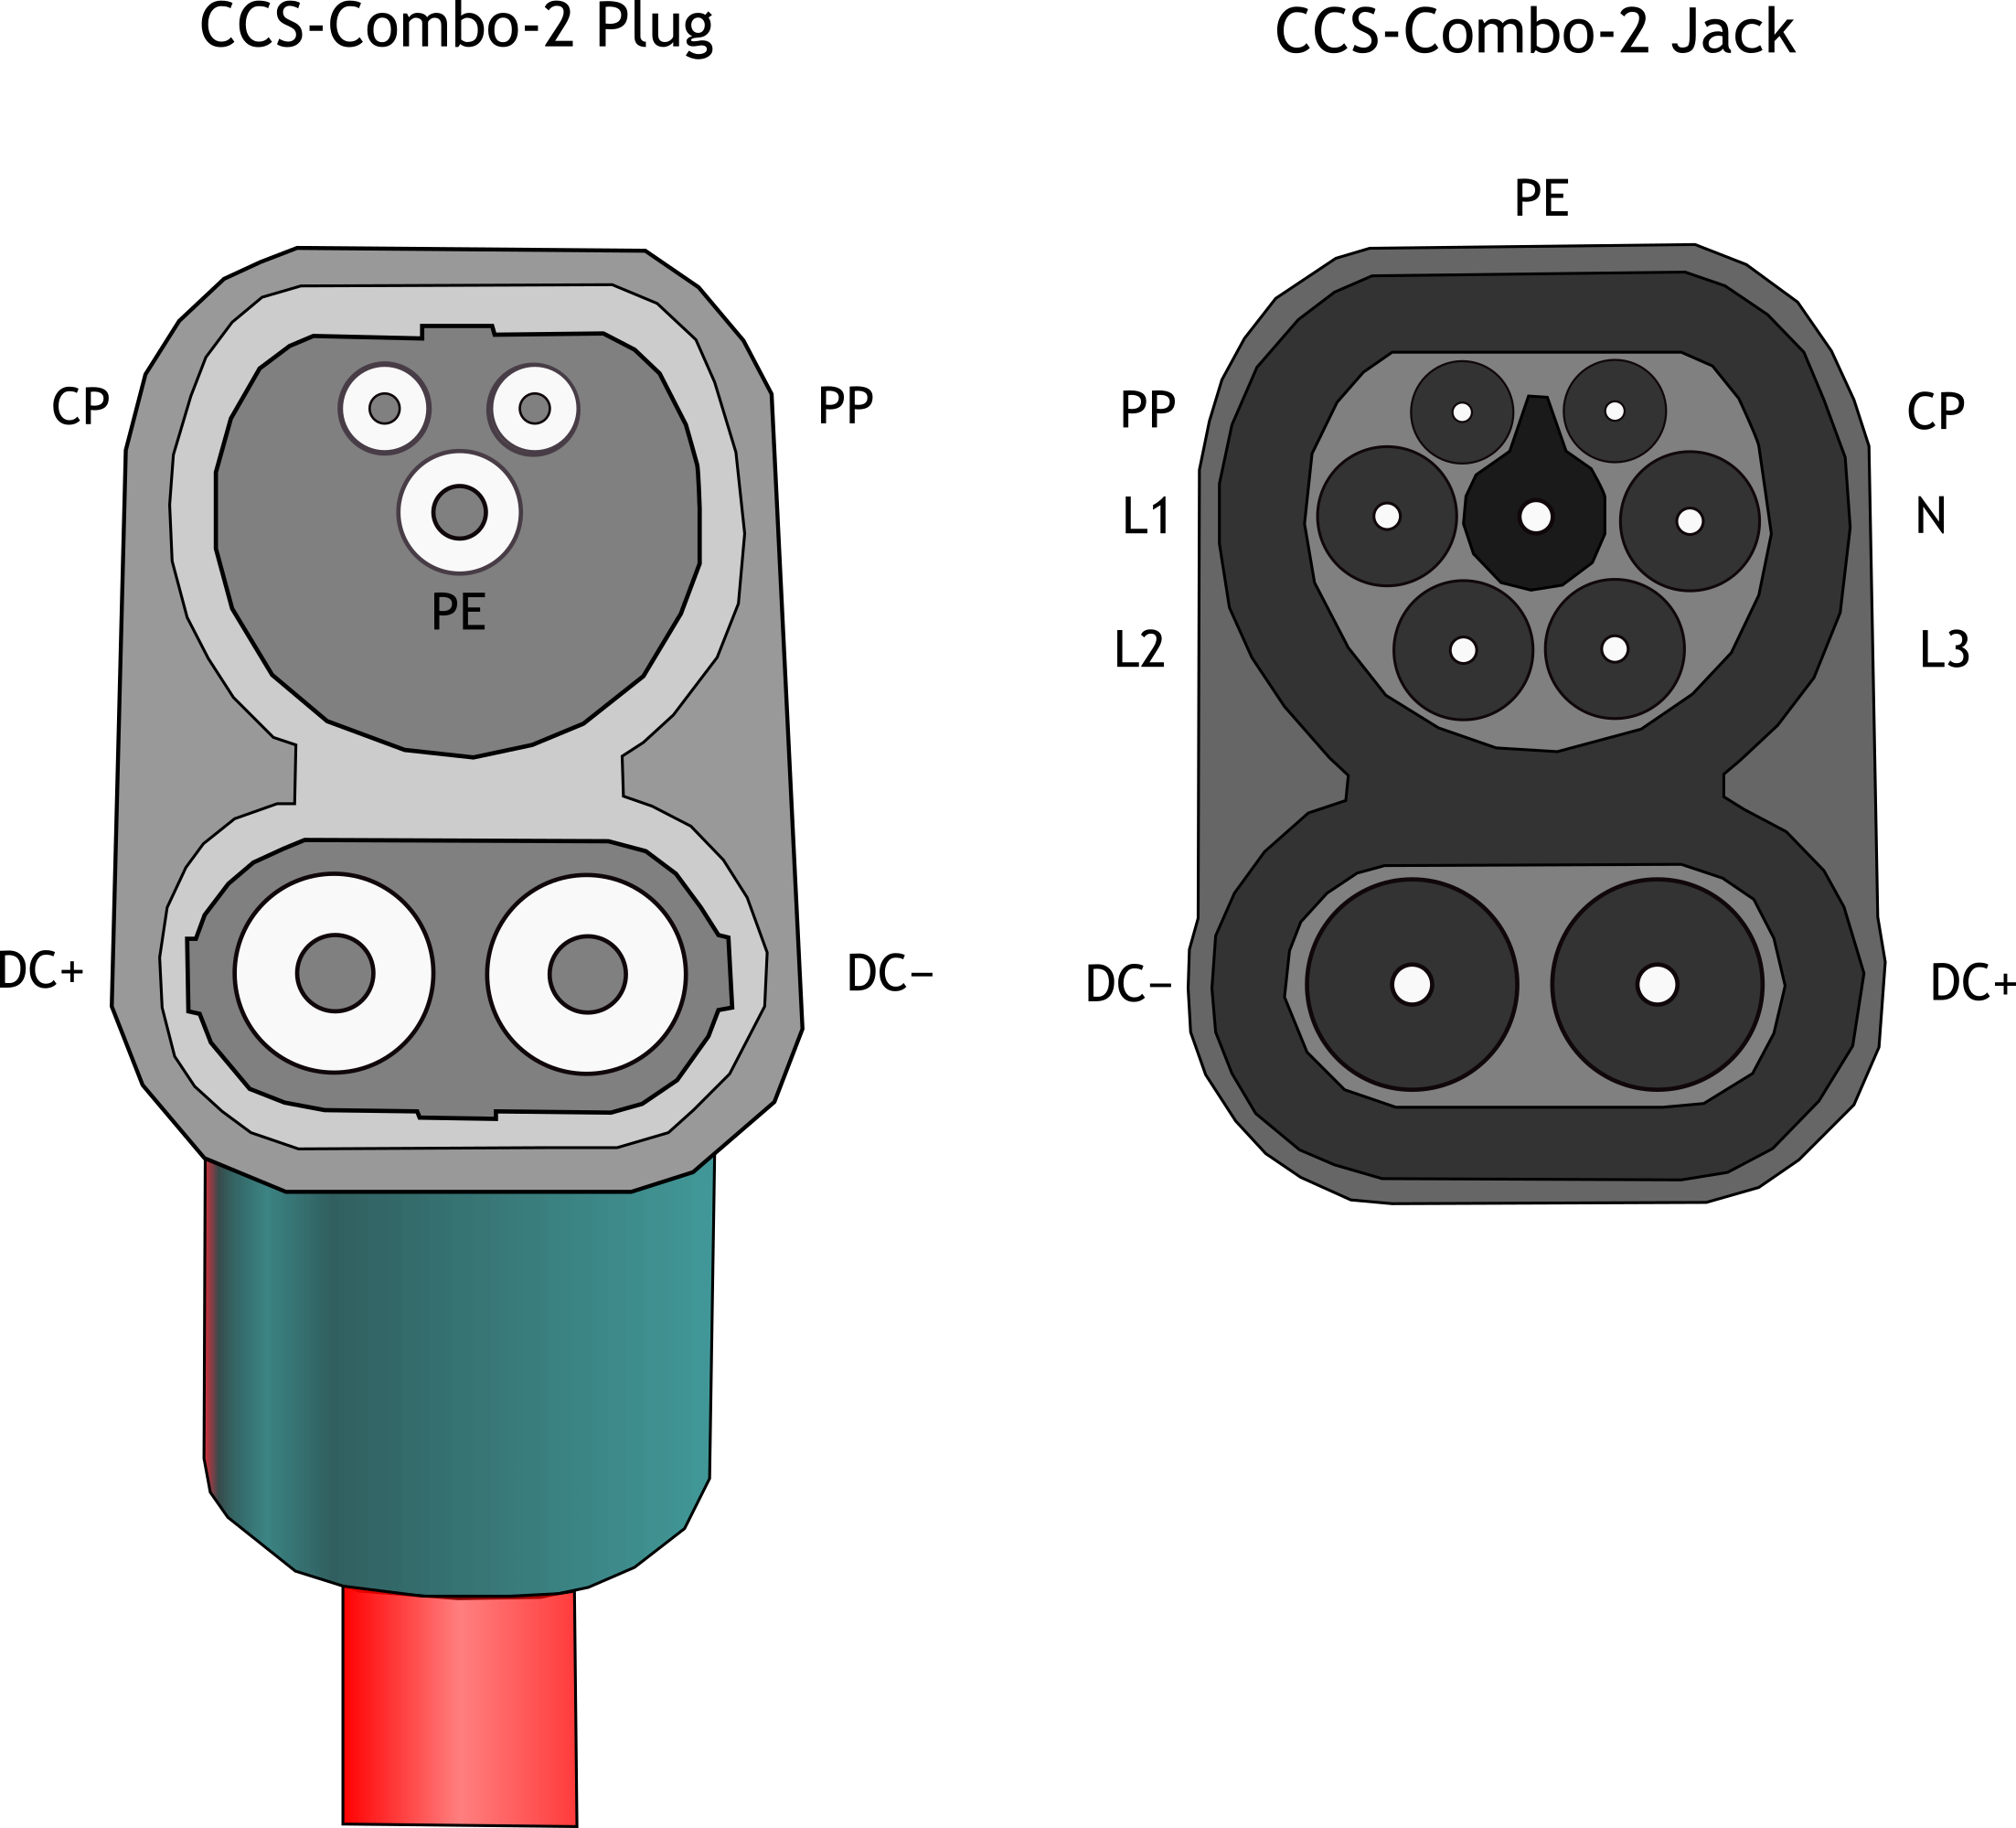
\includegraphics[width=0.7\linewidth]{graphics/CCS-Combo-2.png}
    \caption{Pin assignment of a CCS plug \citep{Ajzh2074-CCS-Plug}}
    \label{fig:CCS-pinout}
    \Description{Pin assignment scheme of a CCS Plug and CCS Jack}
\end{figure}

Two different signaling methods are used to communicate between the EV and the EVSE. First, basic information is exchanged between the EV and the EVSE using pulse width modulation (PWM) via the control pilot (CP). This includes signaling operational readiness and determining the maximum current that can be supplied by the EVSE. This information is transmitted via a PWM signal generated by the EVSE whose duty cycle indicates the available current capacity. In addition, HLC can be requested via a duty cycle of 5\,\%. \citep[pp.\,36--43]{bahrami-ev-2020}

In addition to PWM signaling, Powerline Communication (PLC) is established between the EV and EVSE for further communication. This is based on the HomePlug Green Phy (HPGP) standard, which is a subset of the HomePlug AV standard \citep[p.\,11]{homeplug-green-phy-whitepaper}. The data to be transmitted is modeled on the existing PWM signal between the CP and PE, so no additional data lines are required. A separate PLC modem is installed in both the EV and the EVSE for this communication.

\subsection{Logical Communication Technology}
Once physical communication is established, logical communication layers are set up. These include low-level communication (LLC) with selection of a Central Coordinator (CCo), Signal Level Attenuation Characterization Protocol (SLAC) and formation of a HomePlug AV Logical Network (AVLN), and high-level communication (HLC). The latter establishes communication based on IPv6, TCP/UDP, and other standards. \citep[p.\,49]{bahrami-ev-2020}

\subsubsection{Low-Level Communication}
The HPGP standard creates a logical network, called the HomePlug AV Logical Network (AVLN), for communication so that communication between EV and EVSE is not visible to anyone with access to the line. This requires a central coordinator (CCo) to control the AVLN. In the case of communication between EV and EVSE, the EVSE always assumes the role of CCo. Encrypted messages are then used to communicate in this logical network during the charging process. The required key is exchanged between the EV and the EVSE in the SLAC process. \citep[pp.\,7--8]{homeplug-av-whitepaper}

In addition to exchanging the key for the AVLN, the SLAC process itself also has the function of identifying the closest EVSE to the EV. This is necessary because the PLC can potentially reach multiple charging stations via crosstalk, e.g. via a DC supply bus. To do this, the EV measures the attenuation of the communication to all EVSEs and selects the EVSE with the lowest attenuation. Once the correct EVSE has been identified, the required network membership message is sent in the \texttt{CM\_SLAC\_MATCH.CNF} message, the required Network Membership Key (NMK) and the Network ID (NID) for the AVLN are sent from the EVSE to the EV. The entire SLAC process is shown in Figure \ref{fig:slac-sequence}. \citep[pp.\,49--50]{bahrami-ev-2020} \citep[p.\,16]{homeplug-green-phy-whitepaper}

\begin{figure}[ht]
    \centering
    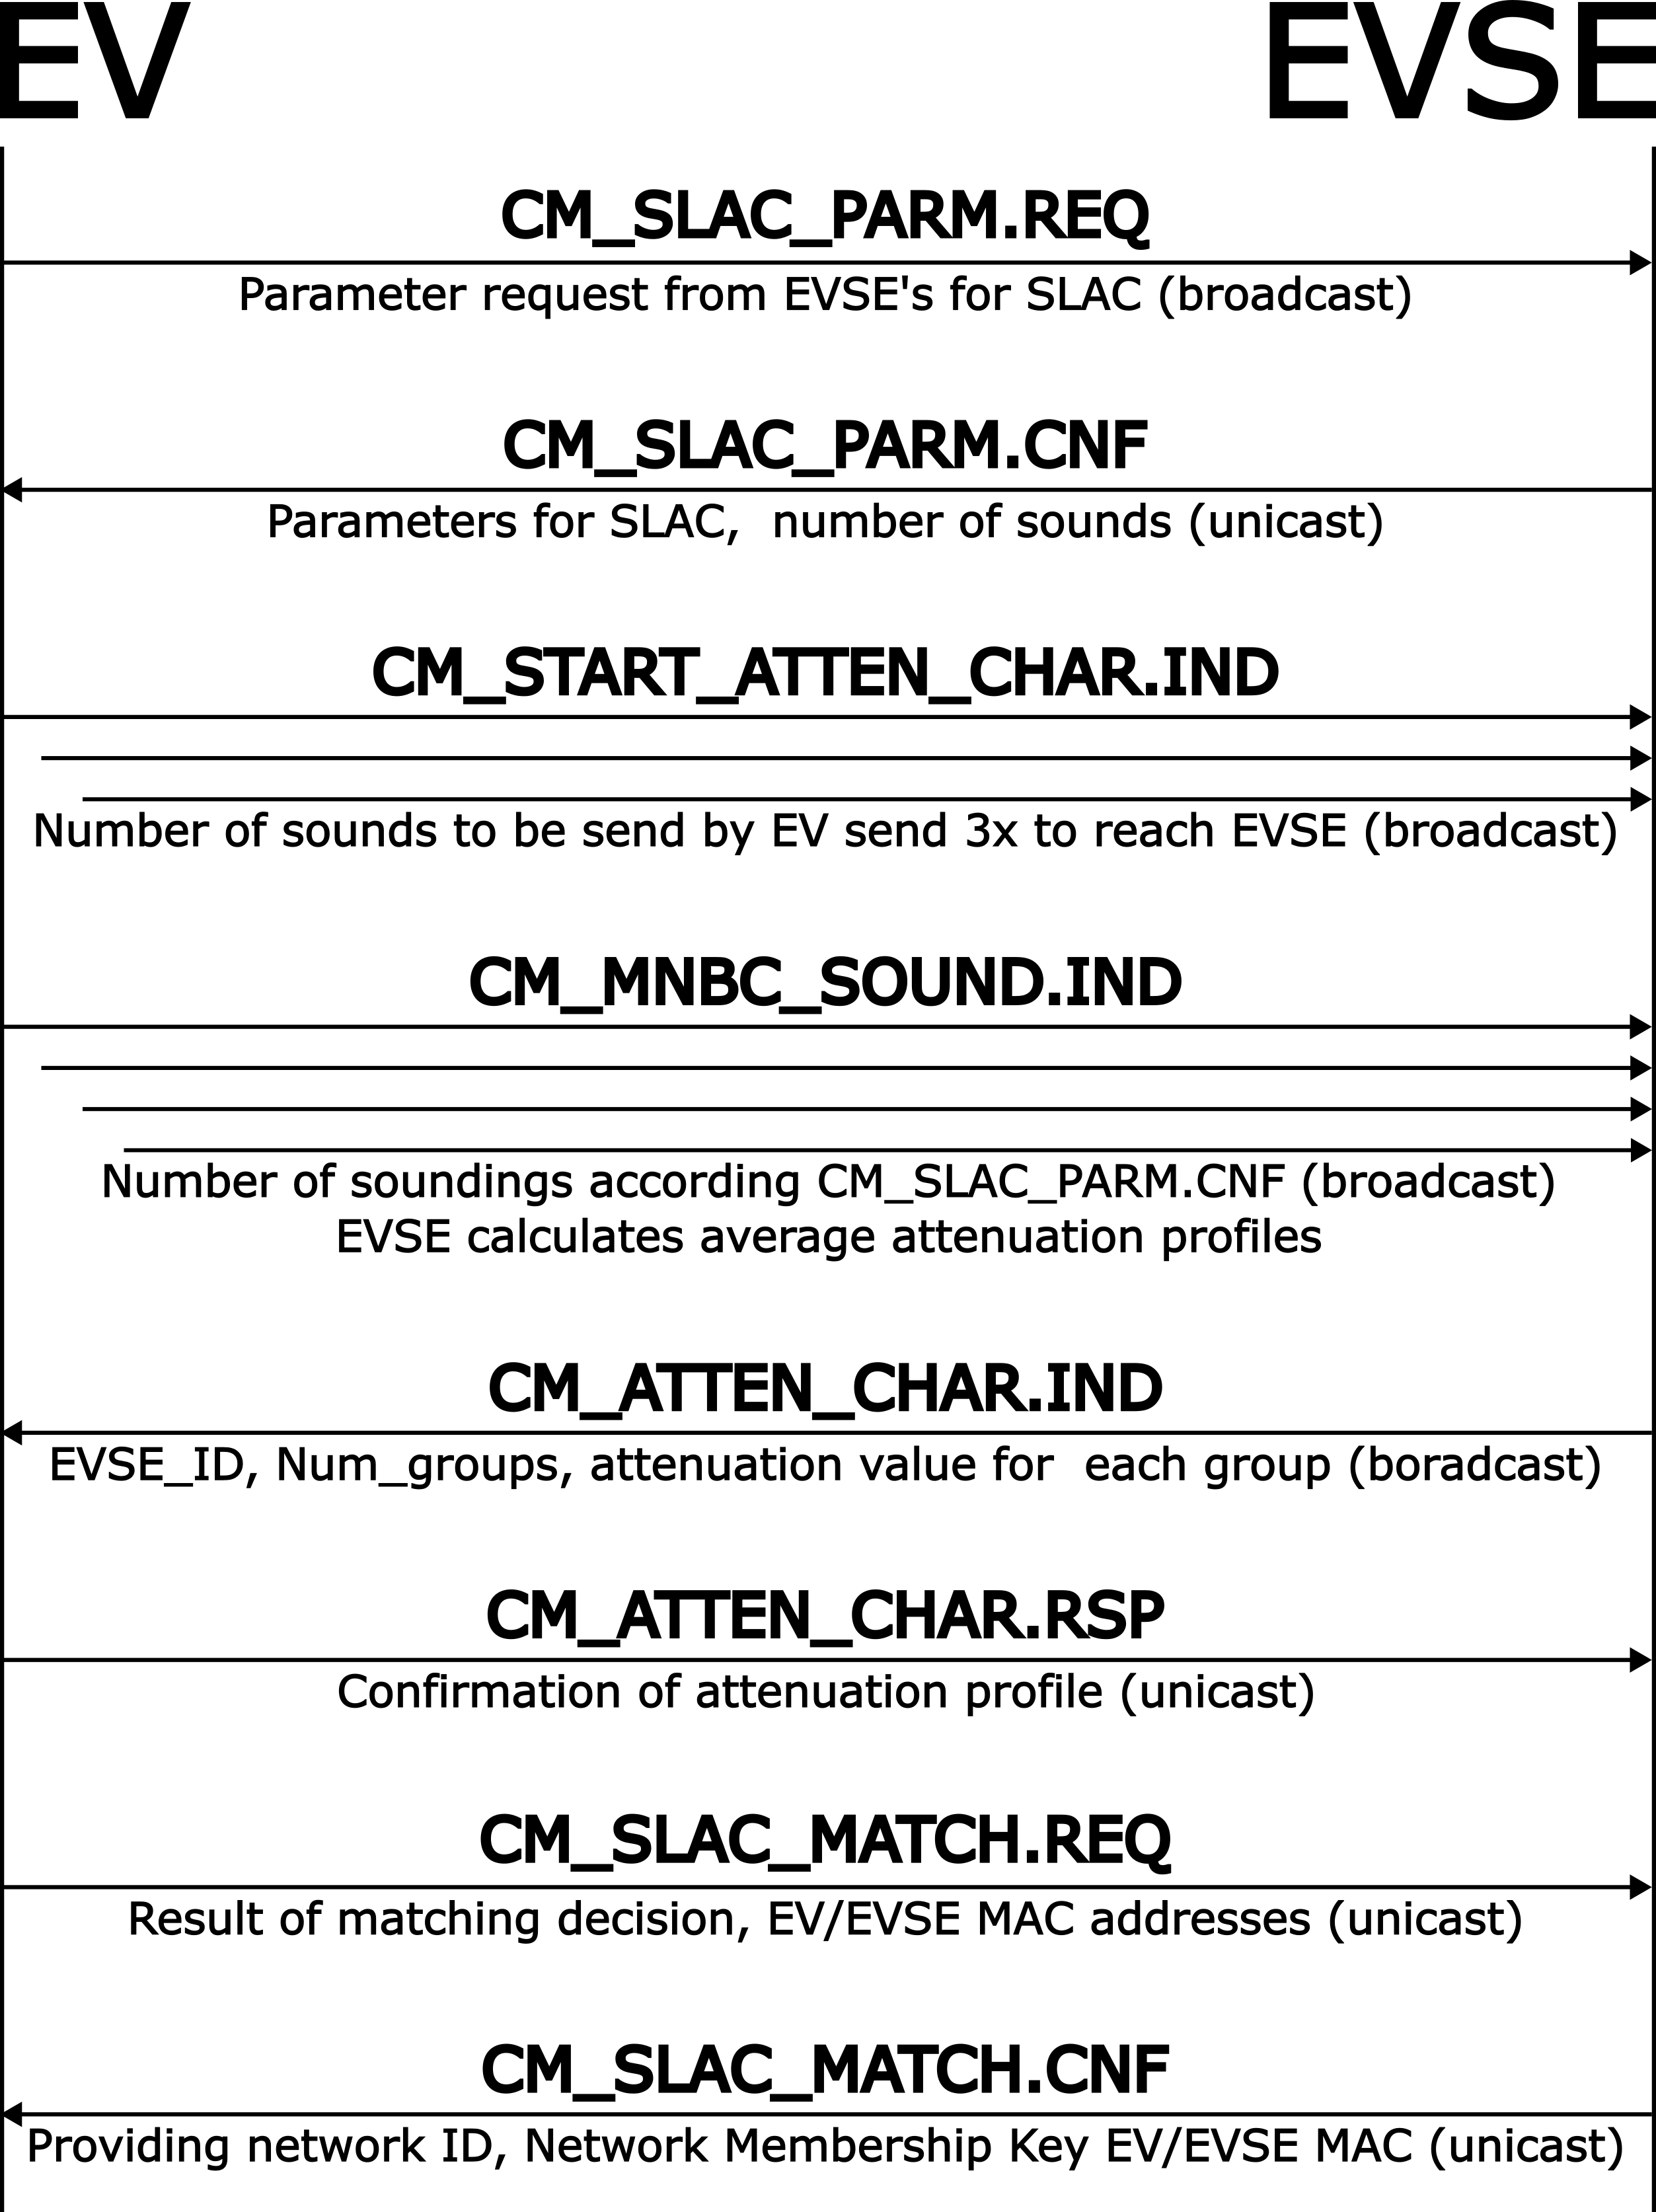
\includegraphics[width=0.7\linewidth]{graphics/SLAC_sequence_slim.png} % {graphics/SLAC_sequence.png}
    \caption{SLAC sequence \citep[p.\,50]{bahrami-ev-2020}}
    \label{fig:slac-sequence}
    \Description{Flow Chart of messages exchanged during the SLAC Process}
\end{figure}

\subsubsection{HLC}
Depending on the type of charging, high-level communication (HLC) can be requested from the EVSE via a PWM signal with a duty cycle of 5\,\%. In this case, the supported protocols are first exchanged using the Service Discovery Protocol (SDP) and a common protocol is defined for subsequent communication. Processes such as payment, encryption, bi-directional charging, and information such as the required voltage or maximum power are exchanged afterwards. In practice, standards such as DIN\,SPEC\,70121, ISO\,15118-2, ISO\,15118-20 or vendor specific protocols are used for this purpose \citep{vector-charging-standards}.

\subsection{Configuration of the Powerline Communication Modem}
The PLC modem requires several parameters to operate. These are set in a Parameter Information Block (PIB) file, which is loaded as the PLC modem boots. This file contains all the information the modem needs to communicate.
It is often necessary to change this configuration. However, the assignment and meaning of the individual bytes is usually unknown, since there is no public documentation available for the PIB files of various modems. Some open source projects, such as open-plc-utils \citep{qcaopen-plc-utils}, HomePlugPWN \citep{fluxiushomeplugpwn}, and others, can help to adjust the files in the correct places, but even here, only a few configuration parameters are known.

\section{Related Work}
The security of communication between EV and EVSE is an active area of research, with several relevant papers investigating attack vectors, vulnerabilities, and possible defenses.

\subsection{Attacks on HomePlug Green PHY and Powerline Communication}
Sébastien Dudek analyzed the HomePlugAV PLC in his paper and demonstrated several attack vectors on PLC networks \citep[pp.\,15--22]{dudek-homeplugav-2015}. The research shows that vulnerabilities in network management and key generation can be exploited to gain access to an AVLN. In addition, the NMK used by an AVLN can be intercepted at the beginning of communication as it is transmitted unencrypted. This implies that an attacker can configure another PLC modem to access the AVLN. This is particularly relevant for charging communication because the HomePlug Green PHY protocol is used for CCS charging, which is potentially vulnerable to similar attacks.

Another paper by Dudek et al. presented the "V2G Injector", a tool to inject data into the communication between an EV and an EVSE \citep[pp.\,24--25]{dudek-v2g-2019}. The tool can modify transmitted data and feed it back into the communication network, allowing it to be used for man-in-the-middle attacks.

\subsection{Brokenwire Attack}
Köhler et al. described the Brokenwire attack, which makes it possible to remotely disrupt ongoing CCS charging processes by deliberately disrupting HomePlug Green PHY PLC communication \citep[pp.\,4--6]{kohler-brokenwire-2022}. The attack exploits the collision detection mechanisms of the Carrier Sense Multiple Access Collision Avoidance (CSMA/CA) protocol to effectively block communication between the EV and the EVSE, which automatically interrupts the charging process. Particularly relevant to this work is the fact, that the PLC used has a high-level of electromagnetic radiation and is susceptible to interference, which can potentially be used to intercept communication.

\subsection{Electromagnetic Sniffing}
Baker and Martinovic showed in their work that the electromagnetic emissions of the PLC signal during CCS charging can be used to wirelessly eavesdrop on the communication between the EV and the EVSE \citep[pp.\,1--2, 7--8]{baker-losing-2019}. They developed a tool for passive detection of HPGP communication that allowed ISO\,15118 messages to be successfully received and decoded depending on the position of the antenna.

They identified a specific vulnerability in the SLAC process where the NMK is transmitted unencrypted \citep[pp.\,9--10]{baker-losing-2019}. This allows an attacker to access the AVLN and read all other data.

They also found that the HPGP encryption is undermined by the unsecured transmission of the NMK and the often missing TLS at public charging stations \citep[pp.\,9--12]{baker-losing-2019}. This means all communication between the EV and the EVSE remains readable to a passive attacker.

\iffalse
Regarding man-in-the-middle attacks, they showed that a fake EVSE could potentially take over and manipulate the entire charging process due to the existing weakness in key management. They suggest securing the SLAC process with elliptic curve encryption to make this attack scenario more difficult \citep[pp.\,17--18]{baker-losing-2019}.

\subsection{Relevance to this Paper}
The work described above shows that both the physical and logical communication between EV and EVSE has several attack vectors. In particular, the HPGP protocol represents a critical vulnerability due to its central role in CCS communication. The communication eavesdropping methods investigated in this thesis are intended to help identify such security risks and evaluate possible countermeasures.
\fi

\section{Passive Sniffing Approaches}
%The purpose of this section is to present the various known approaches to monitoring CCS charging communication. All approaches are presented with their advantages and challenges in order to select the right implementation for different use cases.

Passive sniffing monitors charging communication without interfering with existing communication. This means that neither the EV nor the EVSE communicates directly with the sniffer modem. However, the sniffer modem should be able to receive all messages exchanged between the EV and the EVSE.

The passive monitoring of communication begins with physically recording the data transmitted over the CP and PE lines. This can be accomplished in a laboratory or test environment by modifying the charging cable. At public charging stations, where the charging cable cannot be modified in this way, it is advisable to use a modified adapter plug that allows access to the CP and PE lines.

The tapped lines are next connected to a PLC modem, as shown in Figure \ref{fig:redbeet}. The modem relays messages from the PLC via an Ethernet interface and must be configured as an EV to receive the SLAC messages from the EVSE. Once the Ethernet-equipped modem is connected to a computer, you can use a tool such as Wireshark to analyze the incoming packets.

\begin{figure}[ht]
    \centering
    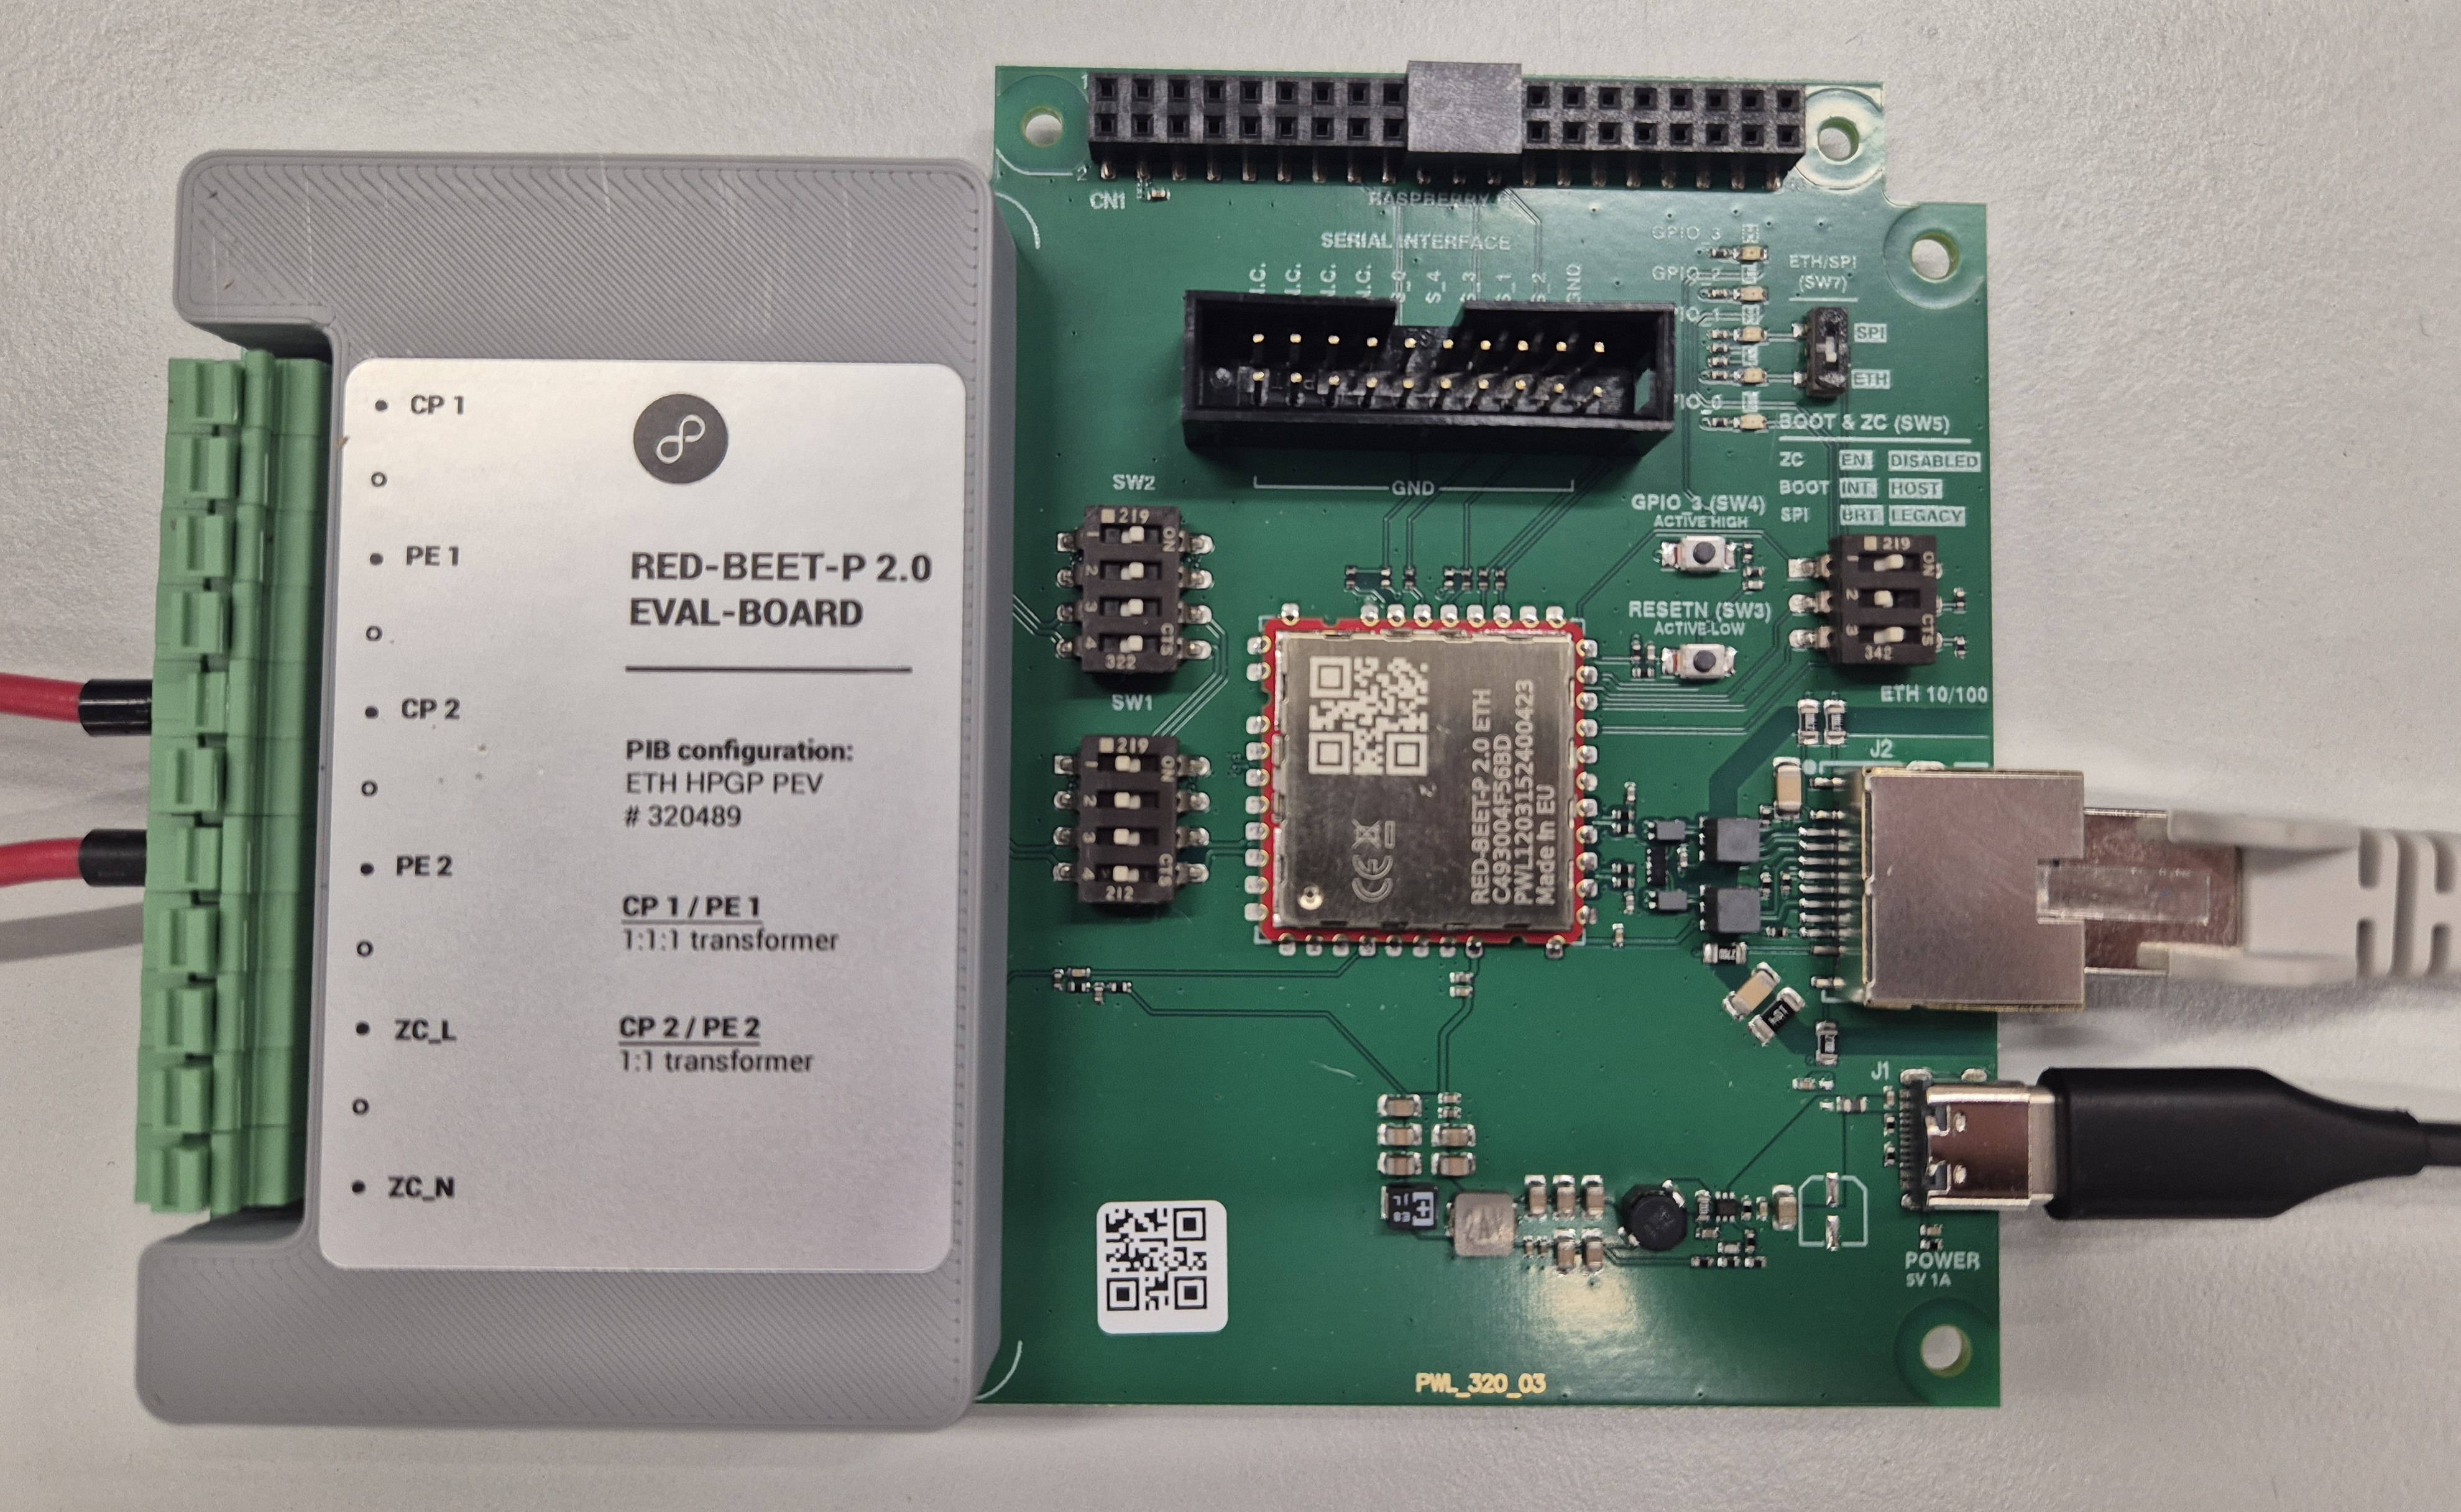
\includegraphics[width=1\linewidth]{graphics/RedBeet-EV.jpg}
    \caption{Sniffer modem with CP and PE cable connected}
    \label{fig:redbeet}
    \Description{Picture of a RED-BEET-P 2.0 EVAL-BOARD with connected CP\,2, PE\,2, Ethernet and Power cables}
\end{figure}

Important data is contained in the \texttt{CM\_SLAC\_MATCH.CNF} message, from which NMK and NID values are extracted and sent in a \texttt{CM\_SET\_KEY.REQ} message to configure the sniffer modem. This allows the modem to join the AVLN and eavesdrop on the charging communication.
% --- Hier erwähnen, dass es zwei SET KEY Nachrichten braucht, bis es funktioniert??? ---

%This approach has the advantage that it can be extended to insert messages as needed. In addition, the simple and inexpensive design allows for implementation in a test environment. However, there are also challenges, especially for public use, where a modified CCS connector or an adapter may be required to access the CP and PE lines.

The main challenge with this approach is that all tested PLC modems act like a layer 2 switch and only forwards broadcast packets and packets for learned participants. For instance, when a packet for destination MAC address $A$ is received on the powerline side, it is only forwarded to the ethernet side, when packets from $A$ have previously been sent from the ethernet side and not from the powerline side.
This means, for a regular charging communication only broadcasts packets, such as SDP requests, can be sniffed. All other packets will be dropped by the modems internal switching logic.

Possible solutions to this problem are discussed in the following sub-items:

\begin{itemize}
    \item Reconfigure the sniffer modem: A possible solution would be to configure the PLC modem to allow all packets from the AVLN to be forwarded over the Ethernet interface, regardless of their destination. However, this would require knowledge of the various configuration parameters, their possible values, and their meaning. Unfortunately, only a few of these are known from open source projects such as \citep{fluxiushomeplugpwn} or \citep{qcaopen-plc-utils}. However, using the known parameters is not sufficient to forward all messages from the AVLN to the Ethernet interface. The problem may be solved with additional information provided by the chip vendor. The vendor however asks for a non-disclosure agreement, which would hinder research and prevent publication of the gained knowledge.
    \item Spoofing approaches: Since, as described above, the PLC modem forwards the messages like a switch, sending spoofed packets with the source MAC address set to the MAC address of the EV or EVSE, tricks the sniffing modem into forwarding packets. However these spoofed packets also affect the swtiching logic of the EVs and EVSEs own modems, causing them to drop packets and interrupting the charging communication.
    %spoofing the MAC address of the EV or EVSE can be used to trick the PLC modem into believing that the corresponding messages need to be forwarded to the Ethernet interface. This can be done, for example, by spoofing IPv6 Neighborhood Solicitation messages. However, the charging communication was interrupted in the tests carried out.
    % ---------- hier evtl no schauen, warum genau des nicht geklappt hat ------------
    % -> Evtl antwortet Modem dann als EV??? - warum gings dann vorher-> war genauso konfiguriert - Trace nomme anschauen - wobei man des da wsl au nich sieht, weils nicht weitergeleitet wird
    % -> Deutet darauf hin, dass auch nicht zwingend komplett passiv - Nicht bekannt, ob PLC Modem Nachrichten über AVLN versendet. Tx Leitung auf Platine abtrennen und damit senden komplett verhindern geht nicht, da Management Botschaften an CCo versendet werden müssen, um dem AVLN beizutreten (https://github.com/uhi22/pyPLC/blob/master/doc/sniffing_experiments.md#q-does-it-help-or-hurt-to-disable-the-physical-transmit-path-to-avoid-that-the-listener-modem-is-involved-into-coordination) - schauen, ob beim kabellosen vom baker auch management Botschaften versendet werden - wenns da ohne geht, muss es ohne gehen.
    \item Manual processing of electrical signals: As an alternative to using available PLC modems and the associated need to configure these modems, an attempt can be made to manually process the electrical signals using a software defined radio, such as GNU Radio \citep{gnuradio}. Such processing has already been investigated in the paper by Baker et al. \citep{baker-losing-2019}. Communication signals were intercepted with an antenna and processed in GNU Radio. The resulting code can be found in \citep{baker-rb-2022}. A disadvantage of this implementation is its complex setup and processing time and therefore makes it impossible to react to messages in real time.
    % --- evtl. hier noch erwähnen, dass des auch gehen müsste - Vector etc. macht des ja auch über ne Antenne und in Echtzeit (glaub ich) - Ist halt wsl nur aufwändiger da extra Hardware dafür zu bauen -----
\end{itemize}

\section{Active sniffing - Man-in-the-Middle}
With man-in-the-middle approaches, all communication is done through the sniffer modem. There are several ways to do this, which are explained below. With all of these methods, all communication is routed through the man-in-the-middle modem. This means that it can potentially modify the messages, insert new messages, or discard messages, which can be very useful for later extensions or other tests.

\subsection{SLAC Man-in-the-Middle}
\label{sec:slac-mitm}
The lowest level approach for a man-in-the-middle attack on charging communication is the exploitation of the SLAC process.
In this process, an attenuation measurement is used to determine the charging station with the best signal quality to avoid communicating with the wrong EVSE due to crosstalk.
As described in \citep[pp.\,8--9]{bao_threat_2018}, this unauthenticated process can be exploited by the attacker, returning a false value for the signal attenuation, thus pretending to be the closest EVSE.
As a result, the EV will consider the attacker modem to be a connected EVSE and send all further requests to that modem.
In order to forward this communication to the real EVSE, a second modem is required, joining the AVLN of the real EVSE, forwarding packets received from the EV to the EVSE and vice versa.

\subsection{SDP Man-in-the-Middle}
\label{sec:sdp-mitm}
After the SLAC process, the EV sends a UDP broadcast based SDP request to negotiate an HLC protocol. According to \citep[p.\,9]{bao_threat_2018}, when an attacker is able to respond to the SDP request faster than the real EVSE it is therefore considered by the EV to be the EVSE. Similar to the previously described approach, the attacker modem can then simply forward all packets received from the EV to the EVSE and vice versa, allowing it to read all communication between the two parties.

\subsection{IPv6 Neighborhood Advertisement Spoofing}
Classic address resolution protocol (ARP) spoofing can also be used in charging communication for active man-in-the-middle attacks.
For ISO\,15118 the communication is based on IPv6, allowing the use of standard IPv6 neighborhood advertisement spoofing tools such as \texttt{parasite6} from \texttt{thc-ipv6} \cite{thcIpv6} or \texttt{sylkie} \cite{sylkie}.
This tricks the EV into thinking a specific IPv6 address is used by the sniffer modems MAC address, allowing to receive and forward packets from the EV to the EVSE and vice versa.

\section{Improving Active Sniffing through Filter Rules}
\label{sec:filter-rules}

The different active man-in-the-middle attack vectors described in the previous section are all based on timing.
For example for the SDP based approach, described in \ref{sec:sdp-mitm}, the charging station might respond with a SDP response faster, resulting in the vehicle connecting to the real charging station rather than the attacker.
Additionally, the vehicle could detect the attack when receiving a second SDP response from a different source.
If an advanced cybersecurity system such as an intrusion detection system would be in place, this would result in the attacker being detected and the communication aborted.

In this section we describe a novel technique utilizing special powerline model features to make man-in-the-middle attacks more reliable.
Since HPGP modems were initially developed as parts of regular network infrastructure just like network switches and hubs, they come with a variety of features, which are not required for charging communication, but rather increase their attack surface.
Our novel approach utilizes \textquotedblleft stream classification rules\textquotedblright\, which are filter rules behaving similar to firewall rules, allowing to drop, alter or redirect packets when their source address, destination address or other attributes match specific values.
According to our tests these filter rules can be configured on target charging stations and electric vehicles from the powerline side.
This means after the attacker modem has joined the powerline network it can configure filter rules both on the vehicle modem and on the charging station modem.

The \texttt{int6krule} tool of the open-plc-utils \citep{qcaopen-plc-utils} can be used to apply filter rules to a PLC modem.
In our tests, we first identified the MAC addresses of the charging station modem as well as the electric vehicle charge controller.
Using these two MAC addresses, we craft the following command:
\begin{lstlisting}
int6krule -i {iface} DropRX Any EthSA Is {pev_mac} add temp {evse_modem_mac}
\end{lstlisting}
where \verb'{iface}' is replaced by the powerline network interface on the attackers computer, \verb'{pev_mac}' by the vehicle MAC address and \verb'{evse_modem_mac}' gets replaced by the charging stations modem address.
This filter rule makes the charging station modem drop all packets originating from the electric vehicle.
This esentially prevents the vehicle to communicate directly to the charging station and most importantly prevents the charging station from receiving the SDP request UDP broadcast packets.
Instead the SDP request is only received by the attacker, which in turn sends its own SDP request to the charging station.
This SDP request is originating from the attackers MAC address and thus is not blocked by the filter rule described above.
This way a charging session between vehicle and attacker and one between attacker and charging station will be established allowing the attacker to read and modify all communication.

When the charging station modem MAC address is not known a similar command can also be crafted for the vehicle side.
For our tests we used a special filter rule allowing to add a VLAN tag to packets.
By adding a VLAN tag to all UDP broadcasts packets originating from the vehicle, the charging station will not be able to receive the SDP request from the vehicle, again allowing the attacker to perform a man-in-the-middle attack.
The command used for this vehicle side filter rule is listed below, replacing \verb'{iface}' like described above and \verb'{pev_modem_mac}' by the MAC address of the vehicles HPGP modem.
\begin{lstlisting}
int6krule -i {iface} -T 8100002a -V 2 TagTX All EthDA Is 33:33:00:00:00:01 add temp {pev_modem_mac}
\end{lstlisting}

\iffalse
% TODO, add more info / details etc.
HPGP Modems can be configured in three different Modes. Unconfigured (to act like a domestic plug), PEV and EVSE. Packet handling, especially for specific HPGP packets, is different for the configured Modes. \citep[p.\,14--15]{dudek-v2g-2019} The Sniffer Modem has to be configured as a PEV to be able to see the necessary \texttt{CM\_SLAC\_MATCH} message from the EVSE.
The \texttt{int6krule} tool of the open-plc-utils \citep{qcaopen-plc-utils} can be used to apply \textquotedblleft stream classification rules\textquotedblright\ to a PLC modem. This means that rules can be set up for the EV and EVSE PLC modems. This option extends and simplifies the SDP man-in-the-middle approach. To do this, a rule is configured on the EVSE to drop all incoming packets from the EV after the SLAC process. Similarly, a rule is configured on the EV to drop all incoming packets from the EVSE. The sniffer modem now has the ability to respond to the EVs SDP request, as was possible in the previous section, without having to be faster than the EVSE. The rest of the behavior is analogous to the previous option and therefore offers the same advantages. The entire HLC can also be listened to here.
\fi

%\section{Hardware Setup and Test Methodology}
% TODO

\section{Open Policy \& Data Access}
The source code of the software used to perform the tests for this work is published on GitHub: \url{https://github.com/securityinmobility/v2g-sniffing/}.

Since the vehicles used for our tests are owned by our or partner research institutes, their identifying information such as vehicle identification numbers and MAC addresses are not considered personal data.
Thus, we published pcapng dumps of high-level communication from all tests with vehicles not owned by individuals on GitHub as well: \url{https://github.com/securityinmobility/vehiclelogs/tree/main/vehicle2grid}
By using the free and open source dissector for V2G communication \texttt{dsV2Gshark}\cite{dspace_dsv2gshark_nodate}, these files can be viewed using Wireshark\cite{wireshark_wireshark_nodate}.

\section{Conclusion}
As shown by this research, charging communication sessions used today can easily be eavesdropped, recorded or altered, when an attacker has physical access to the charging session.

Previous tools for intercepting charging communication were either proprietary or based on unreliable packet timing.
Our novel approach ensures successful interception of charging communication from the first packet.
Additionally the used hardware for our approach is significantly cheaper than all other sniffing devices available today.
This allows researchers to easily debug and reverse engineer ISO\,15118 and other powerline based charging protocols.

Future work might explore the possibilities of utilizing filter rules for attacking charging infrastructure.
For instance the modems allow to permanently store filter rules in non volatile memory opening the possibility to block all traffic originating from any modem and thus possibly disabling the charging station.

With the large amount of features present in todays powerline modems other features might exist, which could additionally be used for attacking charging infrastructure.

%%
%% The acknowledgments section is defined using the "acks" environment
%% (and NOT an unnumbered section). This ensures the proper
%% identification of the section in the article metadata, and the
%% consistent spelling of the heading.
\begin{acks}
This work was created in the research project \textquotedblleft Elektromobiles Sicheres Laden\textquotedblright\ (ESiLa) funded by the Bavarian Ministry of Economic Affairs, Regional Development and Energy under grant DIK0512/01.
\end{acks}

%%
%% The next two lines define the bibliography style to be used, and
%% the bibliography file.
\bibliographystyle{ACM-Reference-Format}
\bibliography{references}


\iffalse
%%
%% If your work has an appendix, this is the place to put it.
\appendix

\section{Research Methods}
\subsection{Part One}
Lorem ipsum dolor sit amet, consectetur adipiscing elit. Morbi
malesuada, quam in pulvinar varius, metus nunc fermentum urna, id
sollicitudin purus odio sit amet enim. Aliquam ullamcorper eu ipsum
vel mollis. Curabitur quis dictum nisl. Phasellus vel semper risus, et
lacinia dolor. Integer ultricies commodo sem nec semper.
\fi

\end{document}
\endinput
%%
%% End of file `sample-sigconf.tex'.
